\section{Transport Layer}
\paragraph{Schicht 4: Transportschicht}

%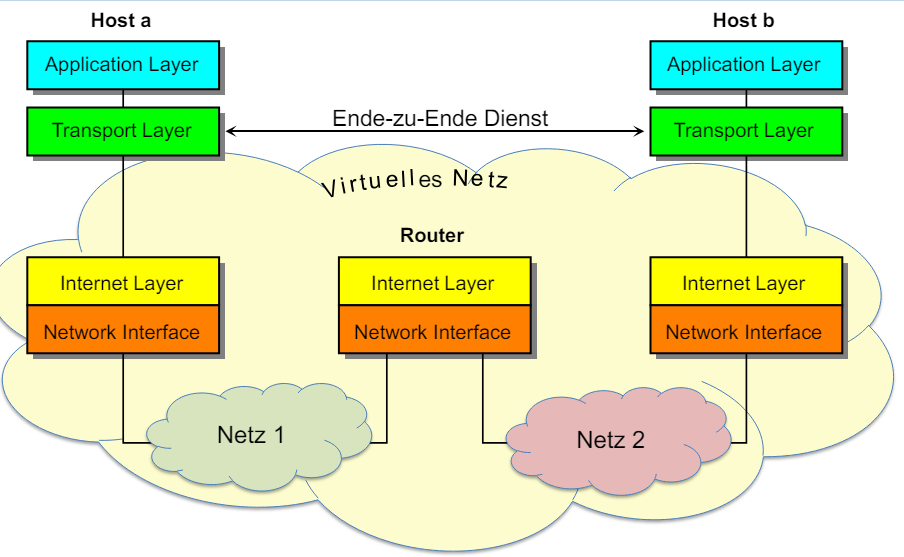
\includegraphics[width=0.75\linewidth]{images/images/transportlayer.png}

\begin{definition}{Transportlayer}
    Schnittstelle zwischen Betriebssystem (Kernel Space) und Anwendungen (User Space)\\
    Zugriff auf Funktionen des Transport Layers erfolgt via klar definierten Schnittstelle (Sockets)
\end{definition}

\begin{definition}{Kapselung} "Protocol" Feld unterscheidet UDP und TCP Daten
    
    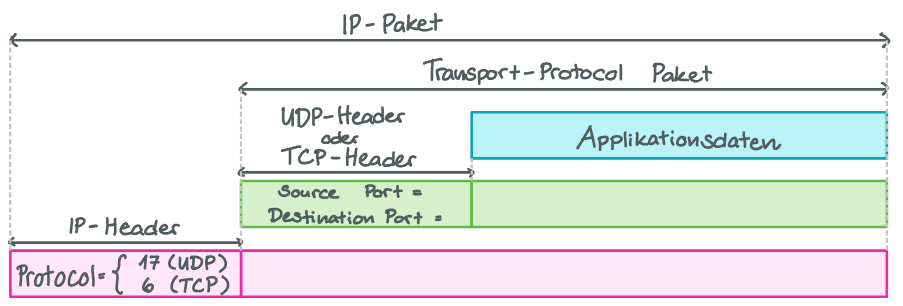
\includegraphics[width=0.9\linewidth]{images/images/tcp_udp_header.png}
\end{definition}

\begin{concept}{Adressierung}\\
    Client adressiert Server-Applikation mit Destination Port Nr.
    \begin{itemize}
        \item sonst weiss TCP/UDP-Modul im Empfänger nicht, welche Applikation gemeint ist
        \item für Source Port Nummer verwendet Client (meist) zufällige Port Nummer >1'023 (vom Betriebssystem vergeben)
    \end{itemize}
\end{concept}

\subsubsection{UDP - User Datagram Protocol}

\begin{definition}{UDP}
    Multi-/Demultiplexen der Datagramme zu Applikationen
    \begin{itemize}
        \item Verbindungslos und unzuverlässig
    \end{itemize}
\end{definition}

\begin{concept}{UDP-Header}
    \begin{itemize}
        \item \textcolor{green}{Source Port} Sendende Applikation
        \item \textcolor{green}{Destination Port} Applikation des Empfängers
        \item \textcolor{blue}{Message Length} Länge des Datagramms
        \item \textcolor{purple}{Checksum} Prüfsumme über einen Pseudo-Header, UDP-Header und Daten (kann Null sein)
        \begin{itemize}
            \item Pseudo-Header: IP Source- und Destination Address, Protocol Feld, Länge des Datagramms
            \begin{itemize}
                \item so können fehlgeleitete Datagramme erkannt werden
            \end{itemize}
        \end{itemize}
    \end{itemize}
        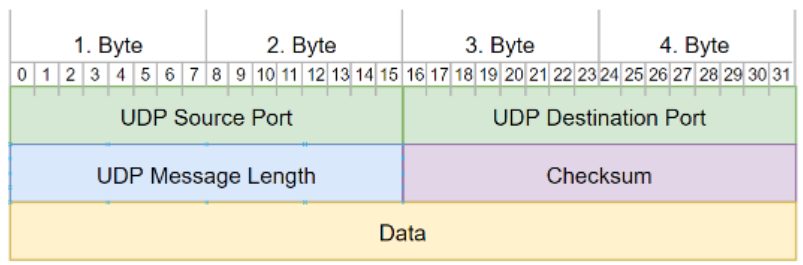
\includegraphics[width=0.9\linewidth]{images/images/udp.png}
\end{concept}

\begin{formula}{Port-Nummern}
    \begin{itemize}
        \item \textcolor{green}{System Ports (Well-Known)} Fix, für bekannte Appl. reserviert
        \item \textcolor{blue}{User Ports (Registered)} Reserviertert für herstellerspez. Appl.
        \item \textcolor{yellow}{Dynamic / Private Ports} Frei verfügbare Ports
    \end{itemize}
        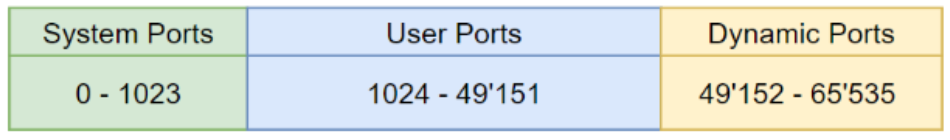
\includegraphics[width=0.8\linewidth]{images/images/portnummern.png}
\end{formula}

\subsubsection{TCP - Transmission Control Protocol}

\begin{definition}{TCP Eigenschaften} 
    Verbindungsorientierte Übertragung, zuverlässiger Verbindungsaufbau, hohe Zuverlässigkeit, Vollduplexübertragung, Stream-Schnittstelle, Graceful Termination, Punkt-zu-Punkt Kommunikation
\end{definition}

\begin{concept}{TCP-Header Format}
    \begin{itemize}
        \item \textcolor{Goldenrod}{Sequence-Nr.} Sicherstellung Reihenfolge der Daten, Erkennung verlorener Daten
        \item \textcolor{Goldenrod}{Acknowledgement-Nr.} n + 1 → Daten bis und mit n korrekt und vollständig angekommen
        \item \textcolor{purple}{Data Offset} Gibt an wo Daten beginnen / enden
        \item \textcolor{purple}{ECN-Flags} Explicit Congestion Notification
        \begin{itemize}
            \item Bit 8: CWR (Congestion Window Reduced)
            \item Bit 9: ECE (ECN-Echo)
        \end{itemize}
        \item \textcolor{purple}{Control Bits} Verbindungsauf- und -abbau (Bits 10-15)\\
        URG: Urgent Pointer\\
        ACK: Acknowledgement Number (Bestätigung empfangener Daten, Erkennung verlorener Daten)\\
        PSH: Push (sofort ohne buffern weiterleiten)\\
        RST: Reset (Verbindung zurücksetzen oder geschlossenen Port signalisieren)\\
        SYN: Verbindungsaufbau,
        FIN: Verbindungsabbau
        \item \textcolor{blue}{Window} Verfügbare Puffergrösse 
        \item \textcolor{purple}{Urgent Pointer} URG = 1 → Position der wichtigen Daten
        \item \textcolor{purple}{Options} Häufigste Verwendung: MSS (Maximum Segment Size) die empfangen werden kann
    \end{itemize}
    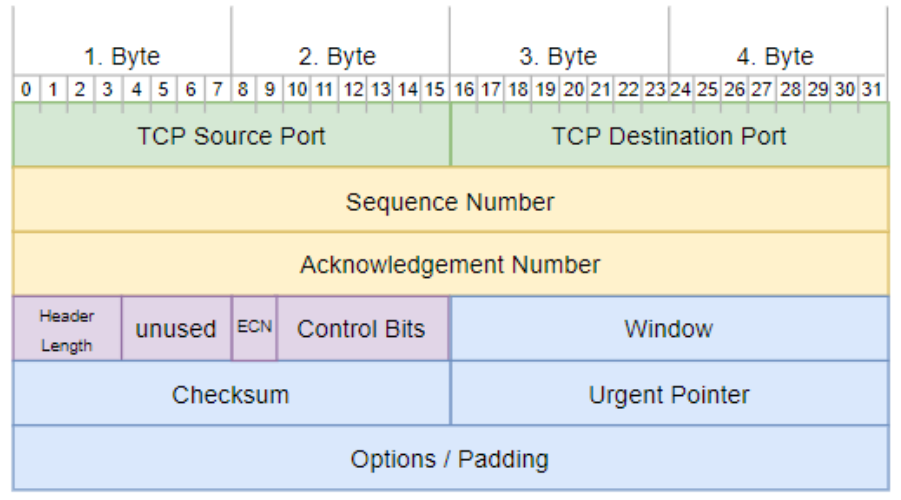
\includegraphics[width=0.9\linewidth]{images/images/tcpheader.png}
\end{concept}

\paragraph{TCP Verkehrssteuerung}

\begin{concept}{Verbindungsorientierte Kommunikation}\\
    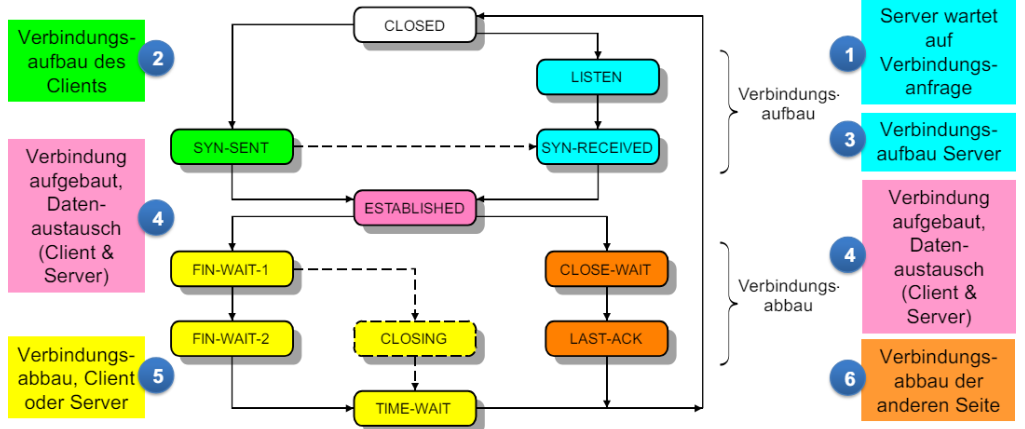
\includegraphics[width=1\linewidth]{images/images/zustandsdiagramm_tcp.png}
\end{concept}

\begin{KR}{Verbindungsaufbau und Verbindungsabbau}\\
\begin{minipage}{0.49\linewidth}
        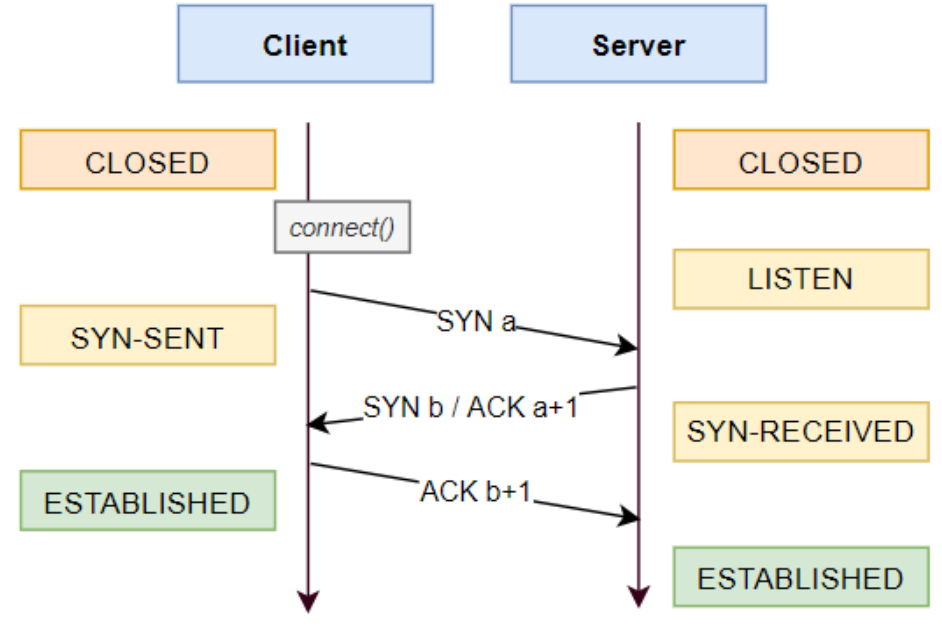
\includegraphics[width=1\linewidth]{images/images/verbindungsaufbau.png}
\end{minipage}
\begin{minipage}{0.5\linewidth}
        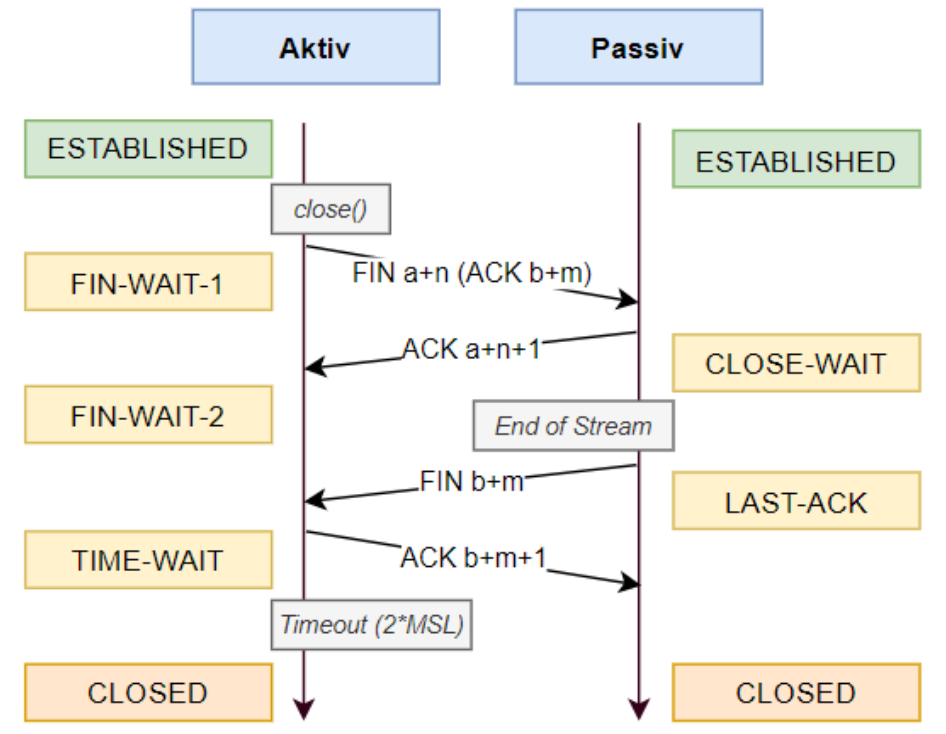
\includegraphics[width=1\linewidth]{images/images/Verbindungsabbau.png}
\end{minipage}

ACK nr. muss mit der Anzahl der Bits der empfangenen Daten aktualisiert werden.
\end{KR}

\paragraph*{Vollständiges Beispiel}

\begin{example}
    Verbindungsaufbau:
    \begin{itemize}
        \item Server „horcht“ (LISTEN) auf einer bestimmten Port Nummer
        \item Client sendet Segment mit SYN=1 und zufälliger init. Sequenznummer a (ACK=0, weil ACK nr. ungültig)
        \item Server bestätigt Sequenznummer mit ACK nr. a+1 und ACK=1, wählt zufällige initiale Sequenznummer b, setzt SYN=1
        \item Client bestätigt b mit ACK nr. b+1 
        \begin{itemize}
            \item Erstes Byte vom Client zum Server hat Sequenznummer a+1
            \item Erstes Byte vom Server zum Client hat Sequenznummer b+1
        \end{itemize}
    \end{itemize}
        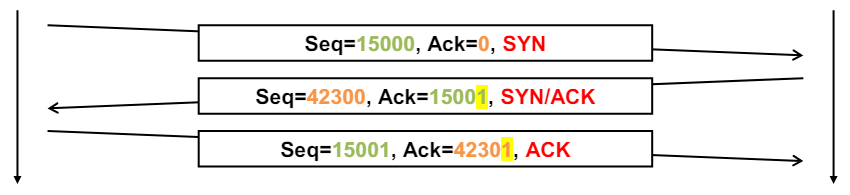
\includegraphics[width=1\linewidth]{images/images/example_verbindungsaufbau_tcp.png}
\end{example}

\begin{example}
    Datenaustausch: TCP-Nachrichten werden bi-direktional ausgetauscht\\
        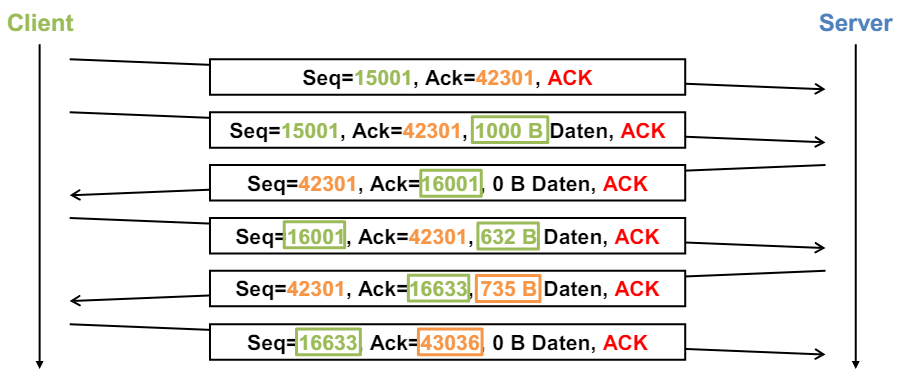
\includegraphics[width=1\linewidth]{images/images/tcp_datenaustausch_ex.png}
\end{example}

\begin{example}
    Beide Seiten können den Verbindungsabbau einleiten
    \begin{itemize}
        \item Ist eine Richtung geschlossen (FIN, ACK), so können in die andere Richtung immer noch Daten gesendet werden (Half-Closed)
        \begin{itemize}
            \item In Richtung der "geschlossenen" Verbindung wird nicht mehr kommuniziert (Acknowledge number mismatch)
        \end{itemize}
        \item Falls die zweite Seite die Verbindung auch schliesst, können die 3. und die 4. Nachricht zusammengefasst werden → FIN/ACK
    \end{itemize}
        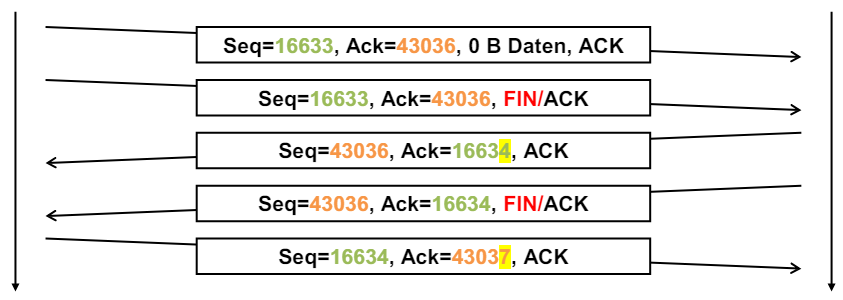
\includegraphics[width=1\linewidth]{images/images/tcp_verbindungsabbau_ex.png}
\end{example}





\subsubsection{TCP Adaptive Elemente}

\begin{formula}{Herausforderungen} zur Zuverlässigkeit zwischen Ethernet/TCP:\\
    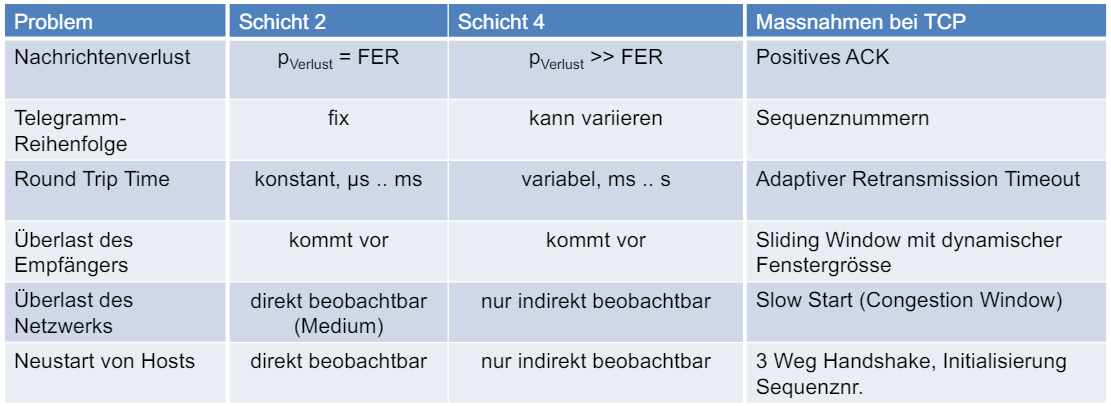
\includegraphics[width=1\linewidth]{images/images/vergleich_layer_2_4.png}
\end{formula}

\paragraph*{Timed Delays}

\begin{formula}{Round Trip Time}
    dynamische Anpassung der Wartezeit 
    $$\alpha = 0.125: \textcolor{blue}{SRTT_n} = (1 - \alpha) \cdot \textcolor{blue}{SRTT_{n-1}} + \alpha \cdot \textcolor{green}{RTT_n}$$
    $$\beta = 0.25: \textcolor{Goldenrod}{RTTVAR_n} = (1 - \beta) \cdot \textcolor{Goldenrod}{RTTVAR_{n-1}} + \beta \cdot \textcolor{blue}{SRTT_n} - \textcolor{green}{RTT_n}|$$
    $$RTO_n = \textcolor{blue}{SRTT_n} + 4 \cdot \textcolor{Goldenrod}{RTTVAR_n}$$
\end{formula}

\begin{formula}{Bandwidth Delay Product (TCP-Puffergrössen)}\\
    \begin{minipage}{0.6\linewidth}
        Wahl der Grösse von Sende- und Empfangspuffer, um Verbindung nicht auszubremsen
        
        \resizebox{\linewidth}{!}{
        $BDP (bits) = RTT (sec) \cdot Bandbreite (bps)$}

        {\footnotesize RTT = Round-Trip-Time}
    \end{minipage}
    \begin{minipage}{0.35\linewidth}
        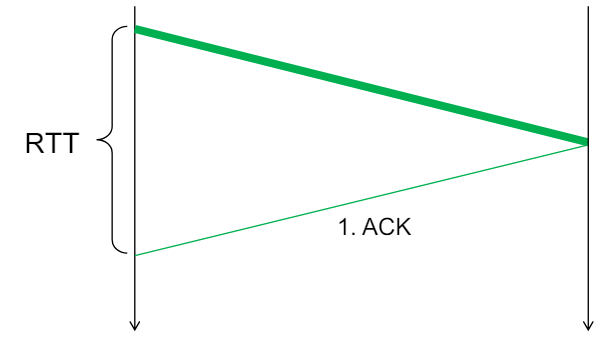
\includegraphics[width=1\linewidth]{images/images/bdp_rtt.png}    
    \end{minipage}
\end{formula}

\paragraph*{Fluss-Steuerung und Congestion Control}

\begin{concept}{Fluss-Steuerung}\\
        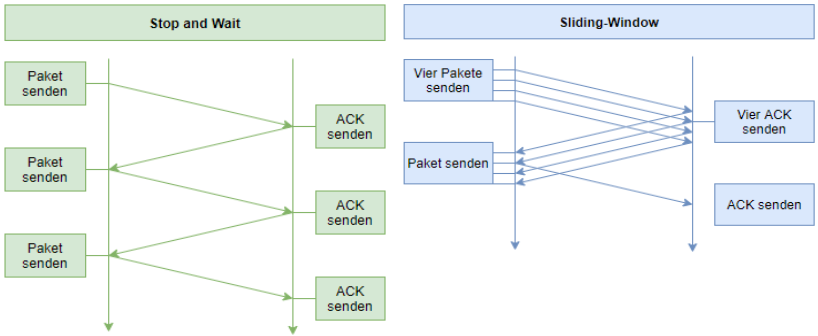
\includegraphics[width=1\linewidth]{images/images/fluss-steuerung.png}
\end{concept}





\begin{KR}{Sliding-Window TCP}
    \begin{itemize}
        \item Beide Richtungen arbeiten unabhängig voneinander
        \item Fenstergrösse wird in Anzahl Bytes angegeben
        \item Verbindungsaufbau: Initiale Fenstergrösse wird der anderen Seite mitgeteilt (Typische Werte: 16 / 32 / 64 KB)
        \item Pufferplatz im Empfänger wird alloziert
        \item Mit jedem ACK wird der verfügbare Pufferplatz (in Bytes) mitgeteilt und damit die Fenstergrösse dynamisch angepasst
        \item Fenstergrösse von 0 Bytes $\rightarrow$ keine Daten mehr senden
        \item Ist im Empfangsbuffer wieder Pufferplatz vorhanden, wird erneut eine Bestätigung mit diesem Pufferplatz an die andere Seite gesendet (= aktuelle Fenstergrösse)
    \end{itemize}
\end{KR}



\begin{example} Sliding Window TCP\\
        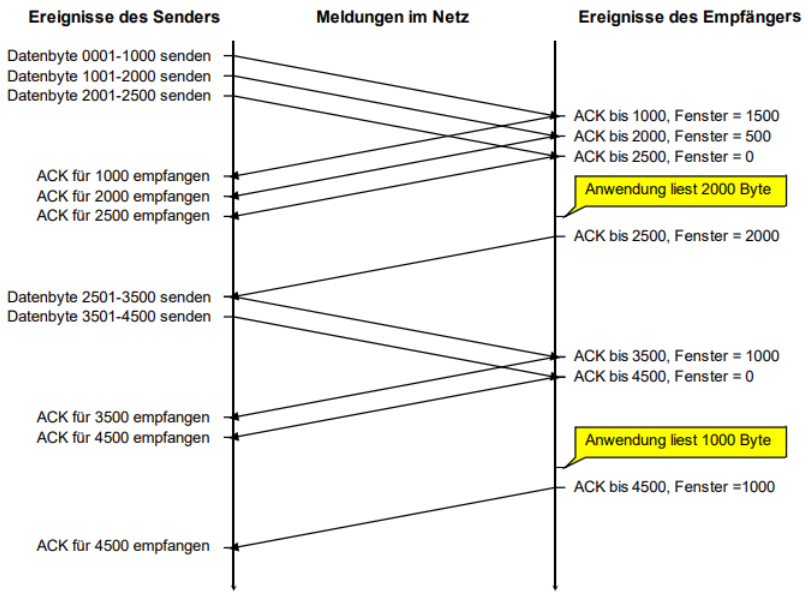
\includegraphics[width=1\linewidth]{images/images/flusssteuerung_tcp.png}\\
    Annahmen: 2'500 Byte Empfangspuffer, 5'000 Bytes Daten
    \begin{itemize}
        \item Fenstergrösse des Empfängers: WindowFeld des TCP-Headers
        \item Wireshark: Advertized Window Size
        \item Sender: nur einen Aufruf von send() für die gesamten 5'000 Bytes
    \end{itemize}
\end{example}

\begin{concept}{Congestion Control - Slow Start}\\
    \begin{minipage}{0.6\linewidth}
        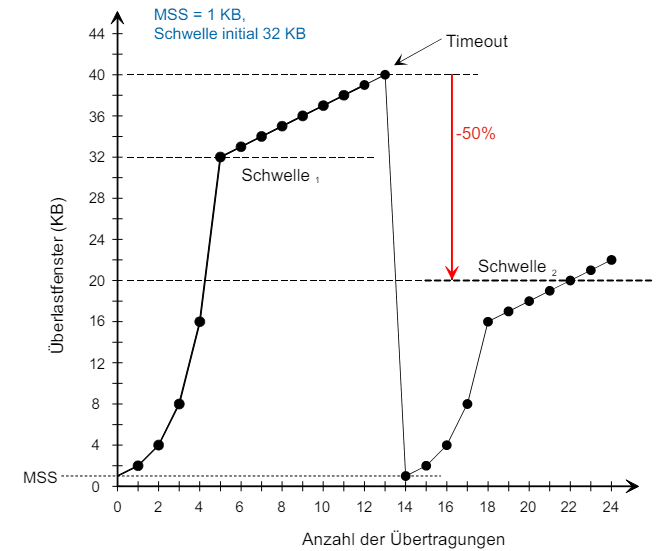
\includegraphics[width=1\linewidth]{images/images/congestion_control.png}
    \end{minipage}
    \begin{minipage}{0.39\linewidth}
        {\small
        Slow Start: herantasten wie gross die einzelnen Frames sein können.

        \vspace{1mm}

        \textcolor{pink}{Wichtig:} Sender kombiniert Congestion Window mit\\ Informationen zur Flow\\ Control vom Empfänger\\ $\rightarrow$ schickt unbestätigte \\Daten bis min\{Congestion\\ Window, Advertised Win.\}\\ erreicht
        }
    \end{minipage}
\end{concept}

